\newpage
\section{Grønland}
I denne afsnit vil Grønland blive beskrevet. Her vil størrelsen af landet, byerne samt bygderne og befolkningstallet blive analyseret.

\subsection{Fakta om Grønland}
\begin{wrapfigure}{l}{0.5\textwidth}
	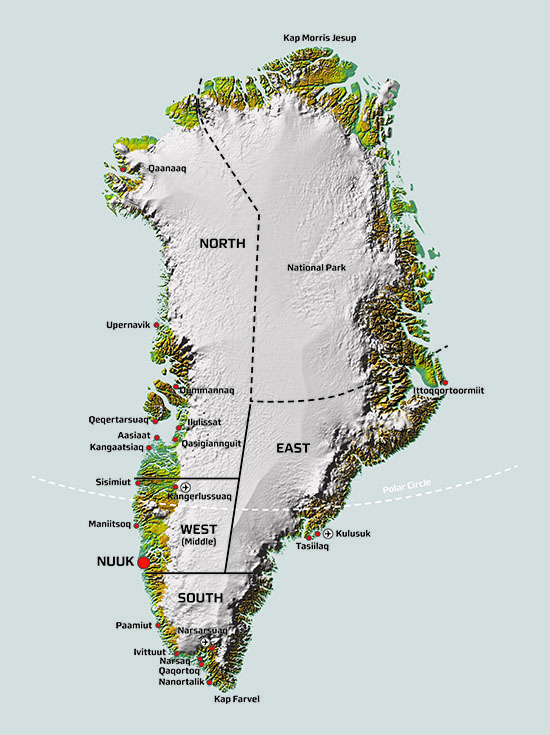
\includegraphics[width=0.5\textwidth]{Figure/greenland.jpg}
	\caption{\textit{Afstandene mellem byerne er store og største delen af Grønland er dækket med is}}
	\label{fig:greenland}
\end{wrapfigure} 
Grønland er verdens største (ikke kontinental) ø \ref{fig:greenland}, som ligger imellem den nordlige Atlantiske Ocean og den Arktiske Hav. Størrelsen af landet er $2.166.086 km^{2}$, hvor $410.449 km^{2}$ er isfrit og kystlinjen strækker sig over 44.000 km. Den isfrie del af Grønland er bjergrig med mange fjorde\cite{grlStat}. \\
Grønland ligger i arktis, det betyder at temperaturen i vinter perioden ligger omkring $-20\deg C$ i den nordligste by og $-3\deg C$ i den sydligste by, hvor imod i sommer perioden ligger temperaturen omkring $7\deg C$ i den nordligste ny og $8\deg C$ i den sydligste by\cite{qaanaaq}\cite{nanortalik}.\\
Den 1. januar 2016 boede der 55.847 personer og grønlands statistik forventer at befolkningsantallet vil falde til 53.000 personer i de kommende 24 år\cite{grlStatWeb}.\\\\
Hovedstaden hedder Nuuk og ligger på grønlands vestkyst, hvor i dag bor omkring 12.800 personer.\\
På tabel \ref{tab:befolkning}, kan befolkningsantallet ses delt i kommunerne.
\newpage
\begin{table}[h]
\centering
    \begin{tabular}{|l|l|}
    \hline
    2016                     & ~      \\ \hline
    Kommune Kujalleq         & 6.811  \\ \hline
    Kommuneqarfik Sermersooq & 22.480 \\ \hline
    Qeqqata Kommunia         & 9.423  \\ \hline
    Qaasuitsup Kommunia      & 17.008 \\ \hline
    Udenfor kommunerne       & 125    \\ \hline
    \end{tabular}
    \caption{Befolkningsantal fordelt i kommuner}
    \label{tab:befolkning}
\end{table}

\subsection{Infrastruktur af telekommunikation}
Som tidligere nævn, er Grønland et stort land, hvor byerne ikke er forbundet med veje, da afstanden mellem byerne og bygderne er stor. Men Tele Greenland har et netværk der forbinder alle byer og bygder i Grønland til omverdenen. Tele Greenland har i dag delt telekommunikationsinfrastrukturen i tre zoner, se figur \ref{fig:zoner}.\\
\begin{figure}[h]
	\centering
	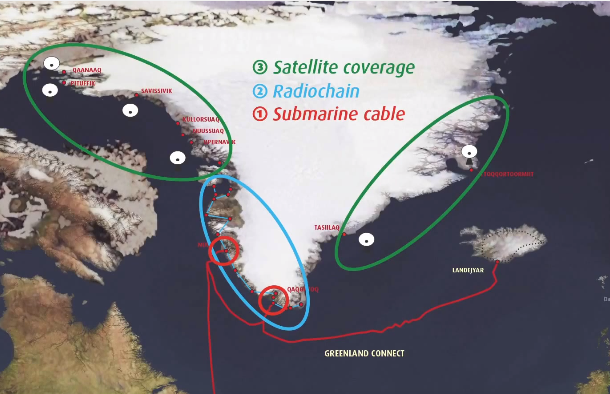
\includegraphics[width=0.8\textwidth]{figure/zoner.PNG}
	\caption{Telekommunikationsinfrastruktur delt i 3 zoner}
	\label{fig:zoner}
\end{figure} 
Den røde linje er søkablet, som er forbundet til to byer i Grønland (Nuuk og Qaqortoq) fra Island og Canada.\\
Den blå cirkel er zonen, hvor byerne og bygderne er forbundet med radiokæde. Cirklen strækker sig fra Nanortalik (Sydgrønland) til Uummannaq (Nordgrønland).\\
Den zone er de grønne cirkler, som er placeret i den nordlige del af Grønland og øst Grønland. byerne og bygderne i de grønne zoner er forbundet til satellitter.\\ 
Den overordnede telekommunikationsinfrastruktur kan ses i bilag \ref{bilag:telesites}\\
De grønne zoner har som sagt kommunikation via satellitter, og derfor er kommunikations hastigheden også ringere end de to andre zoner.

\subsection{Kapacitet}


\subsection{Services}
I de seneste år, viser tallene, at både den mobile bredbånd- og mobiltelefonabonnenter er stigende, hvorimod abonnenter for bredbånd via fastnet og telefonlinjer er faldende.

\subsection{Dataforbrug}

\subsection{Prognose}
I takt med at flere benytter sig af den mobile bredbånd- og mobiltelefonabonnenter, stiger også kapacitetsbehovet for brugerne og kommunikationsnetværket i Grønland.\\
Tele Greenland har udarbejdet en prognose over kapacitetsbehovet over tid (fra 2017 til 2022) og sted i Grønland. 